% THIS IS SIGPROC-SP.TEX - VERSION 3.1
% WORKS WITH V3.2SP OF ACM_PROC_ARTICLE-SP.CLS
% APRIL 2009
%
% It is an example file showing how to use the 'acm_proc_article-sp.cls' V3.2SP
% LaTeX2e document class file for Conference Proceedings submissions.
% ----------------------------------------------------------------------------------------------------------------
% This .tex file (and associated .cls V3.2SP) *DOES NOT* produce:
%       1) The Permission Statement
%       2) The Conference (location) Info information
%       3) The Copyright Line with ACM data
%       4) Page numbering
% ---------------------------------------------------------------------------------------------------------------
% It is an example which *does* use the .bib file (from which the .bbl file
% is produced).
% REMEMBER HOWEVER: After having produced the .bbl file,
% and prior to final submission,
% you need to 'insert'  your .bbl file into your source .tex file so as to provide
% ONE 'self-contained' source file.
%
% Questions regarding SIGS should be sent to
% Adrienne Griscti ---> griscti@acm.org
%
% Questions/suggestions regarding the guidelines, .tex and .cls files, etc. to
% Gerald Murray ---> murray@hq.acm.org
%
% For tracking purposes - this is V3.1SP - APRIL 2009

\documentclass{acm_proc_article-sp}

% 中文断行
\XeTeXlinebreaklocale "zh"
\XeTeXlinebreakskip = 0pt plus 1pt minus 0.1pt

% xetex/xelatex 字体设定宏包
\ProvidesPackage{zhfontcfg}
\usepackage{fontspec,xunicode}
\usepackage{CTEX}
%\defaultfontfeatures{Mapping=tex-text} %如果没有它,会有一些 tex 特殊字符无法正常使用,比如连字符。
\usepackage{algorithm}
\usepackage{algorithmicx}
\usepackage{algpseudocode}

\floatname{algorithm}{算法}
\renewcommand{\algorithmicrequire}{\textbf{输入:}}
\renewcommand{\algorithmicensure}{\textbf{输出:}}

\setCJKmainfont[BoldFont={SimHei}]{SimSun}
\setCJKsansfont{KaiTi}
\setCJKmonofont{DengXian}

\begin{document}

\title{{\fontsize{1em}{\baselineskip}\selectfont 人机对弈五子棋AI程序的设计与实现}}

%
% You need the command \numberofauthors to handle the 'placement
% and alignment' of the authors beneath the title.
%
% For aesthetic reasons, we recommend 'three authors at a time'
% i.e. three 'name/affiliation blocks' be placed beneath the title.
%
% NOTE: You are NOT restricted in how many 'rows' of
% "name/affiliations" may appear. We just ask that you restrict
% the number of 'columns' to three.
%
% Because of the available 'opening page real-estate'
% we ask you to refrain from putting more than six authors
% (two rows with three columns) beneath the article title.
% More than six makes the first-page appear very cluttered indeed.
%
% Use the \alignauthor commands to handle the names
% and affiliations for an 'aesthetic maximum' of six authors.
% Add names, affiliations, addresses for
% the seventh etc. author(s) as the argument for the
% \additionalauthors command.
% These 'additional authors' will be output/set for you
% without further effort on your part as the last section in
% the body of your article BEFORE References or any Appendices.

\numberofauthors{2} %  in this sample file, there are a *total*
% of EIGHT authors. SIX appear on the 'first-page' (for formatting
% reasons) and the remaining two appear in the \additionalauthors section.
%
\author{
% You can go ahead and credit any number of authors here,
% e.g. one 'row of three' or two rows (consisting of one row of three
% and a second row of one, two or three).
%
% The command \alignauthor (no curly braces needed) should
% precede each author name, affiliation/snail-mail address and
% e-mail address. Additionally, tag each line of
% affiliation/address with \affaddr, and tag the
% e-mail address with \email.
%
% 1st. author
\alignauthor
赵乙宁\\
       \affaddr{2017010435}\\
       \email{zhaoyn17@mails.tsinghua.edu.cn}
% 2nd. author
\alignauthor
余齐齐\\
       \affaddr{201801????}\\
       \email{麻烦自己填一下}
}

\maketitle

\begin{abstract}
基于Minimax搜索和$\alpha$-$\beta$优化剪枝的方法,我们编写了一个可进行人机对弈的AI程序。程序从当前状态开始,
依次考虑双方每一种可能动作及其引起的结果状态,对由此产生的状态树进行深度优先的搜索,并使用启发式方法对状态进行估值,和适当
的剪除不必要搜索的分支,从而减小计算量和提高效率。\\
除此之外,我们还使用了散列记录搜索过程中找到的结点的搜索结果,以避免重复搜索相同局面;使用迭代深度搜索方法以充分利用有限的
时间完成尽可能多的搜索,并让浅层的搜索结果为高层的搜索提供子节点搜索顺序的参考。
根据五子棋的特点,我们还引入了一种特别的搜索顺序和剪枝方法,优先搜索距离前几步下棋位置近的结点、剪除距离任何现有棋子都很远
的结点,以进一步降低搜索树的平均分支数,加快搜索效率、加深在有限时间内可以搜索到的层数。
最后,我们在现有框架的基础上加入了悔棋和复盘的功能,丰富了游戏的提示文字、完善了输入检查,以增强人类玩家使用本程序的体验。\\
在实验环境下,我们的程序可以在$5s$内搜索平均$2.5\times10^6$个结点,对状态树完整地完成$4-6$层的搜索。程序在与人类的实际对战中
也取得了良好的效果,有时可以提前6-10回合就找到制胜的策略。\\
       \\
       \\
\end{abstract}

\section{\textbf{概述}}
博弈在人类社会中广泛存在,小到人与人之间的棋牌类游戏,大到整个金融、资本和贸易市场的运行,都存在着各种各样的博弈问题。
博弈问题也是现代人工智能研究的重点问题之一,经过长期的发展,人们已经研究出了许多种有利于解决博弈问题的算法,其中重要的一种
就是对抗搜索。\\
经典的对抗搜索适用于完全可观测的、确定性的、离散性的博弈问题,通过把问题建模成多个参与方共同进行动作影响游戏状态,并最终产
生一个结果的模型,把问题的每个状态和状态之间的可转移关系建模为状态树来模拟真实世界的博弈过程,通过从初始状态开始按一定的策
略来搜索状态树以在有限的计算资源下寻求对自己最有利的方案。\\
一种常用的对抗搜索方法是Minimax搜索,即通过交替模拟双方可以采取的可行动作,在决定己方动作时总是选择所有动作中带来效用(或启发
式函数产生的预估效用)最大的一个,在预测对方动作时总是选择所有动作中带来效用最大的一个,这样不仅符合对抗博弈问题的基本逻辑,
而且使得智能体能够正确评估预测自己的行为在一定时期之后能产生的结果,避免贪心搜索带来的过分陷入局部最优的问题。
另外重要的一点是,由于Minimax搜索中上层结点的结果总是取决于下层结点的结果的最大值或最小值,因此我们可以采用一种名为
$\alpha-\beta$优化剪枝的方法,当下层结点发现自己返回最终的结果已经不可能成为上层结点的最值、被上层结点选用时,就提前结束
本层的搜索。这样可以大大的降低Minimax方法嗖嗖的分支数,提高搜索的效率。\\
由于五子棋的每一个状态结点下,对当前行动的一方而言在任何一个空位置下棋都是合法的行动,五子棋问题的搜索树的平均分支数量极高,
可以达到近200,而游戏结束往往需要30-60轮行动,因而即使使用了各种剪枝方法也几乎不可能一次性搜索到最终游戏结束对应的结点状态,
因此基于启发函数评估局面的限定深度搜索是必须的。根据五子棋的特点,我们使用了一套启发式评估方法,它评估双方在场上拥有的活二、
活三、冲三、活四、冲四等棋型的数量,并以此为依据对局面做出预估。\\
$\alpha-\beta$搜索的特点决定了其剪枝的效果受搜索结点的先后顺序的影响十分严重。对每一结点的的搜索过程,其需要循环搜索自己的
各个所有子节点、计算子节点的结果;这一过程中足够好的子结点越是先被搜索出来,则搜索自己的余下子节点的过程就能够得到更好的剪
枝,$\alpha-\beta$优化剪枝就能发挥更好的作用。因此决定循环搜索子结点的顺序就成为了十分重要的问题。\\
由于考虑到在实际问题中智能体做出决策的时间往往是受限的,我们利用迭代深度搜索的方法,通过限定实际搜索所用的时间、不
固定搜索进行的层数,让搜索进行的层数随着搜索的过程不断迭代增加,从而使智能体可以最大限度的利用所给的时间进行尽可能深入的搜
索、找到尽可能好的答案;利用散列表优化的方法,通过在搜索过程中把在某一结点上得到的结果存储进散列表中,使得后面的搜索过程不
必重复搜索之前已经搜索过的状态。但更重要的是这两种方法的结合使用使得我们在进行更深层的搜索时,能够根据对这个状态结点之前进
行浅层搜索时找到的最佳结果的记忆,优先搜索这个结点。因为在进行深层搜索时找到的最佳结果在搜索树上的路径,有很大可能是仍然沿
着之前浅层搜索时找到的最佳路径的,这样就达到了让最好的子结点更可能被最先搜索出来的目的,从而优化了$\alpha-\beta$优化剪枝的
效果。\\
除此之外,根据五子棋的特点,我们还引入了一种特别的搜索顺序决定方法和优化剪枝方法:在决定搜索顺序时按照某一空位置距离前几个
回合下棋的位置的距离排序、尽量让距离前几个回合下棋位置近的节点被优先的搜索,和剪除对距离棋盘上任何棋子距离都较远的位置的搜
索,我们可以进一步的优化搜索顺序,和在不明显损伤智能体强度的情况下降低搜索树平均分支数量,从而达到提高搜索效率、加深搜索层
数的目的。\\
我们的程序基于给定的五子棋框架开发,实现了输入输出、落子合法性判断、胜负判断等人机对弈程序所需要的基本功能,并额外实现了悔
棋、复盘等附加功能,丰富了游戏内的文字提示和对用户的输入进行完善的合法性检查,以给人类玩家使用本程序带来更好的体验。\\

我们的方法主要有以下几个部分:
\begin{enumerate}
       \item Minimax搜索和$\alpha-\beta$优化剪枝
       \item 评估局面的启发式函数的设计与实现
       \item 散列表优化和迭代深度搜索
\end{enumerate}

一般的下棋经验告诉我们,在大多数情况下,效用高的下棋位置要么是
进攻的,即延长自己已经有的连珠,使其接近五连珠;要么是防守的,即破坏、截断对手的连珠,避免其在未来成为五连珠。无论哪种情况
,我们都往往应该在自己现有的棋子周边或对方现有的棋子周边下棋,而一般不会在距离任何现有棋子都很远的位置下棋;在概率意义上,的通过剪除对距离棋盘上任何现有棋子距离都很远的空位置的搜索
(这样的位置往往是不会得到很大的收益的),从而进一步降低每个搜索结点的平均分枝数,以加快搜索效率、加深在有限时间内可以搜索到的层数。\\

\section{\textbf{方法}}

\subsection{\textbf{程序基本框架}}
总体上程序可以分为两个部分:通用五子棋运行逻辑部分和AI智能体部分。详细的文件模块介绍如表1所示。\\
\begin{table*}
       \centering
       \caption{文件模块一览表}
       \begin{tabular}{|c|c|l|} \hline
       所属部分 & 文件名(不含扩展名) & 说明\\ \hline
       运行逻辑 & define & 定义各类基础的游戏数据结构如棋盘、点、行棋记录、启发式估值等\\ \hline
       运行逻辑 & start & 游戏主循环,控制复盘、存盘、读取人类和AI的动作输入、打印棋盘等\\ \hline
       运行逻辑 & makemove & 解析控制台输入,获取AI输入,验证合法性,进行下棋,撤销下棋\\ \hline
       运行逻辑 & gameover & 判断游戏是否结束和胜负\\ \hline
       运行逻辑 & printchessboard & 把棋盘打印在控制台上\\ \hline
       AI & evaluate & 对一个完整游戏状态进行局面估值\\ \hline
       AI & createmoves & 产生所有的可行动作和循环遍历时的先后顺序构成的有序列表\\ \hline
       AI & searchmove & 对局面进行递归的、迭代深度的Minimax搜索和$\alpha-\beta$优化剪枝\\ \hline
       AI & hashsearch & 定义散列表,提供接口计算局面的键值、修改和查询散列表中的数据\\ \hline
       AI & cutoffTest & 判定是否停止搜索子节点、调用启发式函数对局面进行估值\\ \hline
       AI & stopSearchSiblingsTest & 判定是否因$\alpha-\beta$或超时等,对未搜索的子结点进行剪枝\\ \hline
       \end{tabular}
\end{table*}\\
% end the environment with {table*}, NOTE not {table}!
通用五子棋逻辑部分循环地从控制台读取人类玩家的输入、调用AI智能体部分提供的接口获取AI的输入,对他们的输入进行合法性验证后操
作棋盘下棋、判断游戏是否结束,并控制棋盘的打印、悔棋、存盘、复盘等操作。\\
AI智能体部分为通用五子棋运行逻辑部分提供一个接口,接受某一时刻的棋盘等游戏状态信息,并返回一个AI此时希望下棋的位置。\\
此外还有部分开发过程中更好的测试启发式函数的结果或AI决策的结果所用的文件,它们在Release模式下不会被链接进主程序因此下文不
再叙述。\\

\subsection{\textbf{Minimax搜索和$\alpha-\beta$优化剪枝}}
基本的Minimax搜索方法是用递归函数来实现的,在我们的程序中对应于searchmove.cpp的SearchStep函数。\\
AI智能体部分对外提供一个接口SearchMove(),它返回一个Point结构体。Point结构体的定义如下:
\begin{quote}
       struct Point \{\\
       \hspace*{0.6cm} int x;\\
       \hspace*{0.6cm} int y;\\
       \}
\end{quote}
SearchMove()函数没有形参,但是会读取define.h中定义的游戏棋盘、当前玩家、游戏历史记录等数据,组合成GameFullStatus类的对象,
并将其的引用传递给SearchStep函数,由此开始对状态树的根节点(即当前局面)的搜索。相关定义如下:
\begin{quote}
       struct LegalMove \{\\
       \hspace*{0.6cm} //表示当前局面下当前的玩家的一个合法的下棋行动,包括下棋的位置和这个位置的优先级\\
       \hspace*{0.6cm} Point p;\\
       \hspace*{0.6cm} int priority = 0;//这个位置点对应的优先级,越低则越应当被首先搜索。
       \};\\
       \\
       class GameFullStatus \{\\
       public:
       \hspace*{0.6cm} int player; // 当前要行动的玩家编号\\
       \hspace*{0.6cm} int (*board)[GRID_NUM]; // 当前棋盘\\
       \hspace*{0.6cm} vector<pair<int, Point>> playHistory;//下棋的历史记录\\
       \hspace*{0.6cm} unsigned long long zobrist;\\
       \\
       \hspace*{0.6cm}inline bool putChess(const LegalMove &move);\\
       \hspace*{0.6cm}inline bool unputChess(const LegalMove &move);\\
       \};
\end{quote}
\qquad MinimaxWe ha \qquad ve alrea \qquad dy seen several typeface changes in this sample.  You
can indicate italicized words or phrases in your text with
the command \texttt{{\char'134}textit}; emboldening with the
command \texttt{{\char'134}textbf}
and typewriter-style (for instance, for computer code) with
\texttt{{\char'134}texttt}.  But remember, you do not
have to indicate typestyle changes when such changes are
part of the \textit{structural} elements of your
article; for instance, the heading of this subsection will
be in a sans serif\footnote{A third footnote, here.
Let's make this a rather short one to
see how it looks.} typeface, but that is handled by the
document class file. Take care with the use
of\footnote{A fourth, and last, footnote.}
the curly braces in typeface changes; they mark
the beginning and end of
the text that is to be in the different typeface.

You can use whatever symbols, accented characters, or
non-English characters you need anywhere in your document;
you can find a complete list of what is
available in the \textit{\LaTeX\
User's Guide}\cite{Lamport:LaTeX}.

\subsection{Math Equations}
You may want to display math equations in three distinct styles:
inline, numbered or non-numbered display.  Each of
the three are discussed in the next sections.

\subsubsection{Inline (In-text) Equations}
A formula that appears in the running text is called an
inline or in-text formula.  It is produced by the
\textbf{math} environment, which can be
invoked with the usual \texttt{{\char'134}begin. . .{\char'134}end}
construction or with the short form \texttt{\$. . .\$}. You
can use any of the symbols and structures,
from $\alpha$ to $\omega$, available in
\LaTeX\cite{Lamport:LaTeX}; this section will simply show a
few examples of in-text equations in context. Notice how
this equation: \begin{math}\lim_{n\rightarrow \infty}x=0\end{math},
set here in in-line math style, looks slightly different when
set in display style.  (See next section).

\subsubsection{Display Equations}
A numbered display equation -- one set off by vertical space
from the text and centered horizontally -- is produced
by the \textbf{equation} environment. An unnumbered display
equation is produced by the \textbf{displaymath} environment.

Again, in either environment, you can use any of the symbols
and structures available in \LaTeX; this section will just
give a couple of examples of display equations in context.
First, consider the equation, shown as an inline equation above:
\begin{equation}\lim_{n\rightarrow \infty}x=0\end{equation}
Notice how it is formatted somewhat differently in
the \textbf{displaymath}
environment.  Now, we'll enter an unnumbered equation:
\begin{displaymath}\sum_{i=0}^{\infty} x + 1\end{displaymath}
and follow it with another numbered equation:
\begin{equation}\sum_{i=0}^{\infty}x_i=\int_{0}^{\pi+2} f\end{equation}
just to demonstrate \LaTeX's able handling of numbering.

\subsection{Citations}
Citations to articles \cite{bowman:reasoning, clark:pct, braams:babel, herlihy:methodology},
conference
proceedings \cite{clark:pct} or books \cite{salas:calculus, Lamport:LaTeX} listed
in the Bibliography section of your
article will occur throughout the text of your article.
You should use BibTeX to automatically produce this bibliography;
you simply need to insert one of several citation commands with
a key of the item cited in the proper location in
the \texttt{.tex} file \cite{Lamport:LaTeX}.
The key is a short reference you invent to uniquely
identify each work; in this sample document, the key is
the first author's surname and a
word from the title.  This identifying key is included
with each item in the \texttt{.bib} file for your article.

The details of the construction of the \texttt{.bib} file
are beyond the scope of this sample document, but more
information can be found in the \textit{Author's Guide},
and exhaustive details in the \textit{\LaTeX\ User's
Guide}\cite{Lamport:LaTeX}.

This article shows only the plainest form
of the citation command, using \texttt{{\char'134}cite}.
This is what is stipulated in the SIGS style specifications.
No other citation format is endorsed.

\subsection{Tables}
Because tables cannot be split across pages, the best
placement for them is typically the top of the page
nearest their initial cite.  To
ensure this proper ``floating'' placement of tables, use the
environment \textbf{table} to enclose the table's contents and
the table caption.  The contents of the table itself must go
in the \textbf{tabular} environment, to
be aligned properly in rows and columns, with the desired
horizontal and vertical rules.  Again, detailed instructions
on \textbf{tabular} material
is found in the \textit{\LaTeX\ User's Guide}.

Immediately following this sentence is the point at which
Table 1 is included in the input file; compare the
placement of the table here with the table in the printed
dvi output of this document.

\begin{table}
\centering
\caption{Frequency of Special Characters}
\begin{tabular}{|c|c|l|} \hline
Non-English or Math&Frequency&Comments\\ \hline
\O & 1 in 1,000& For Swedish names\\ \hline
$\pi$ & 1 in 5& Common in math\\ \hline
\$ & 4 in 5 & Used in business\\ \hline
$\Psi^2_1$ & 1 in 40,000& Unexplained usage\\
\hline\end{tabular}
\end{table}

To set a wider table, which takes up the whole width of
the page's live area, use the environment
\textbf{table*} to enclose the table's contents and
the table caption.  As with a single-column table, this wide
table will ``float" to a location deemed more desirable.
Immediately following this sentence is the point at which
Table 2 is included in the input file; again, it is
instructive to compare the placement of the
table here with the table in the printed dvi
output of this document.


\begin{table*}
\centering
\caption{Some Typical Commands}
\begin{tabular}{|c|c|l|} \hline
Command&A Number&Comments\\ \hline
\texttt{{\char'134}alignauthor} & 100& Author alignment\\ \hline
\texttt{{\char'134}numberofauthors}& 200& Author enumeration\\ \hline
\texttt{{\char'134}table}& 300 & For tables\\ \hline
\texttt{{\char'134}table*}& 400& For wider tables\\ \hline\end{tabular}
\end{table*}
% end the environment with {table*}, NOTE not {table}!

\subsection{Figures}
Like tables, figures cannot be split across pages; the
best placement for them
is typically the top or the bottom of the page nearest
their initial cite.  To ensure this proper ``floating'' placement
of figures, use the environment
\textbf{figure} to enclose the figure and its caption.

This sample document contains examples of \textbf{.eps}
and \textbf{.ps} files to be displayable with \LaTeX.  More
details on each of these is found in the \textit{Author's Guide}.

\begin{figure}
\centering
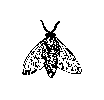
\epsfig{file=fly.eps}
\caption{A sample black and white graphic (.eps format).}
\end{figure}

\begin{figure}
\centering
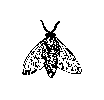
\epsfig{file=fly.eps, height=1in, width=1in}
\caption{A sample black and white graphic (.eps format)
that has been resized with the \texttt{epsfig} command.}
\end{figure}


As was the case with tables, you may want a figure
that spans two columns.  To do this, and still to
ensure proper ``floating'' placement of tables, use the environment
\textbf{figure*} to enclose the figure and its caption.

Note that either {\textbf{.ps}} or {\textbf{.eps}} formats are
used; use
the \texttt{{\char'134}epsfig} or \texttt{{\char'134}psfig}
commands as appropriate for the different file types.

\subsection{Theorem-like Constructs}
Other common constructs that may occur in your article are
the forms for logical constructs like theorems, axioms,
corollaries and proofs.  There are
two forms, one produced by the
command \texttt{{\char'134}newtheorem} and the
other by the command \texttt{{\char'134}newdef}; perhaps
the clearest and easiest way to distinguish them is
to compare the two in the output of this sample document:

This uses the \textbf{theorem} environment, created by
the\linebreak\texttt{{\char'134}newtheorem} command:
\newtheorem{theorem}{Theorem}
\begin{theorem}
Let $f$ be continuous on $[a,b]$.  If $G$ is
an antiderivative for $f$ on $[a,b]$, then
\begin{displaymath}\int^b_af(t)dt = G(b) - G(a).\end{displaymath}
\end{theorem}

The other uses the \textbf{definition} environment, created
by the \texttt{{\char'134}newdef} command:
\newdef{definition}{Definition}
\begin{definition}
If $z$ is irrational, then by $e^z$ we mean the
unique number which has
logarithm $z$: \begin{displaymath}{\log e^z = z}\end{displaymath}
\end{definition}

\begin{figure}
\centering
\psfig{file=rosette.ps, height=1in, width=1in,}
\caption{A sample black and white graphic (.ps format) that has
been resized with the \texttt{psfig} command.}
\end{figure}

Two lists of constructs that use one of these
forms is given in the
\textit{Author's  Guidelines}.

\begin{figure*}
\centering
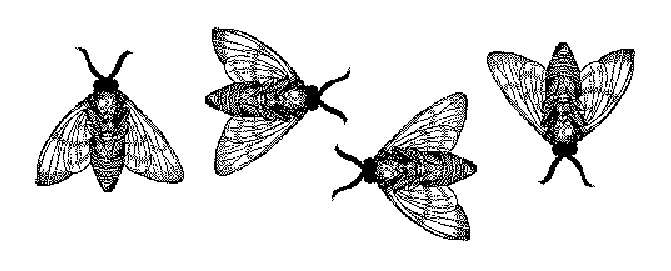
\epsfig{file=flies.eps}
\caption{A sample black and white graphic (.eps format)
that needs to span two columns of text.}
\end{figure*}
and don't forget to end the environment with
{figure*}, not {figure}!

There is one other similar construct environment, which is
already set up
for you; i.e. you must \textit{not} use
a \texttt{{\char'134}newdef} command to
create it: the \textbf{proof} environment.  Here
is a example of its use:
\begin{proof}
Suppose on the contrary there exists a real number $L$ such that
\begin{displaymath}
\lim_{x\rightarrow\infty} \frac{f(x)}{g(x)} = L.
\end{displaymath}
Then
\begin{displaymath}
l=\lim_{x\rightarrow c} f(x)
= \lim_{x\rightarrow c}
\left[ g{x} \cdot \frac{f(x)}{g(x)} \right ]
= \lim_{x\rightarrow c} g(x) \cdot \lim_{x\rightarrow c}
\frac{f(x)}{g(x)} = 0\cdot L = 0,
\end{displaymath}
which contradicts our assumption that $l\neq 0$.
\end{proof}

Complete rules about using these environments and using the
two different creation commands are in the
\textit{Author's Guide}; please consult it for more
detailed instructions.  If you need to use another construct,
not listed therein, which you want to have the same
formatting as the Theorem
or the Definition\cite{salas:calculus} shown above,
use the \texttt{{\char'134}newtheorem} or the
\texttt{{\char'134}newdef} command,
respectively, to create it.

\subsection*{A {\secit Caveat} for the \TeX\ Expert}
Because you have just been given permission to
use the \texttt{{\char'134}newdef} command to create a
new form, you might think you can
use \TeX's \texttt{{\char'134}def} to create a
new command: \textit{Please refrain from doing this!}
Remember that your \LaTeX\ source code is primarily intended
to create camera-ready copy, but may be converted
to other forms -- e.g. HTML. If you inadvertently omit
some or all of the \texttt{{\char'134}def}s recompilation will
be, to say the least, problematic.

\section{Conclusions}
This paragraph will end the body of this sample document.
Remember that you might still have Acknowledgments or
Appendices; brief samples of these
follow.  There is still the Bibliography to deal with; and
we will make a disclaimer about that here: with the exception
of the reference to the \LaTeX\ book, the citations in
this paper are to articles which have nothing to
do with the present subject and are used as
examples only.
%\end{document}  % This is where a 'short' article might terminate

%ACKNOWLEDGMENTS are optional
\section{Acknowledgments}
This section is optional; it is a location for you
to acknowledge grants, funding, editing assistance and
what have you.  In the present case, for example, the
authors would like to thank Gerald Murray of ACM for
his help in codifying this \textit{Author's Guide}
and the \textbf{.cls} and \textbf{.tex} files that it describes.

%
% The following two commands are all you need in the
% initial runs of your .tex file to
% produce the bibliography for the citations in your paper.
\bibliographystyle{abbrv}
\bibliography{sigproc}  % sigproc.bib is the name of the Bibliography in this case
% You must have a proper ".bib" file
%  and remember to run:
% latex bibtex latex latex
% to resolve all references
%
% ACM needs 'a single self-contained file'!
%
%APPENDICES are optional
%\balancecolumns
\appendix
%Appendix A
\section{Headings in Appendices}
The rules about hierarchical headings discussed above for
the body of the article are different in the appendices.
In the \textbf{appendix} environment, the command
\textbf{section} is used to
indicate the start of each Appendix, with alphabetic order
designation (i.e. the first is A, the second B, etc.) and
a title (if you include one).  So, if you need
hierarchical structure
\textit{within} an Appendix, start with \textbf{subsection} as the
highest level. Here is an outline of the body of this
document in Appendix-appropriate form:
\subsection{Introduction}
\subsection{The Body of the Paper}
\subsubsection{Type Changes and  Special Characters}
\subsubsection{Math Equations}
\paragraph{Inline (In-text) Equations}
\paragraph{Display Equations}
\subsubsection{Citations}
\subsubsection{Tables}
\subsubsection{Figures}
\subsubsection{Theorem-like Constructs}
\subsubsection*{A Caveat for the \TeX\ Expert}
\subsection{Conclusions}
\subsection{Acknowledgments}
\subsection{Additional Authors}
This section is inserted by \LaTeX; you do not insert it.
You just add the names and information in the
\texttt{{\char'134}additionalauthors} command at the start
of the document.
\subsection{References}
Generated by bibtex from your ~.bib file.  Run latex,
then bibtex, then latex twice (to resolve references)
to create the ~.bbl file.  Insert that ~.bbl file into
the .tex source file and comment out
the command \texttt{{\char'134}thebibliography}.
% This next section command marks the start of
% Appendix B, and does not continue the present hierarchy
\section{More Help for the Hardy}
The acm\_proc\_article-sp document class file itself is chock-full of succinct
and helpful comments.  If you consider yourself a moderately
experienced to expert user of \LaTeX, you may find reading
it useful but please remember not to change it.
\balancecolumns
% That's all folks!
\end{document}
